\section{From a ring to a line}\label{sec:line}

Write $a_n=(a_{n,1},\ldots,a_{n,n})$ for the marks in $[0,M]$ and
$R_n$ for the infimum central radius with outer radii $N_n a_{n,i}$,
where $N_n>0$. A zero mark is a point on the central circle and imposes
no angular separation. For $R>0$ the cosine law gives the required
angle between a pair of outer radii $u,v$ as
\begin{equation}\label{eq:theta}
 \theta_R(u,v)=2\asin\sqrt{\frac{uv}{(R+u)(R+v)}}
 =2\atan\sqrt{\frac{uv}{R(R+u+v)}}.
\end{equation}
Both cyclic arcs between the pair must subtend at least this angle,
since the smaller angle belongs to $[0,\pi]$. For positive radii the
angle is symmetric, positive, increasing in each outer radius and
strictly decreasing in $R$. In a cyclic order $\sigma=(u_1,\ldots,u_n)$
of positive radii with $n\ge3$, the sum of adjacent angles decreases
continuously from $n\pi$ to zero. Its unique root at level $2\pi$ is
$\ch(\sigma)$, the adjacent-chain closure radius. Summing the adjacent
constraints gives $\ch(\sigma)\le\full(\sigma)$, where $\full(\sigma)$
is the least feasible radius in that order.

\begin{definition}\label{def:line}
For a finite list $a=(a_1,\ldots,a_N)$ in $[0,M]$, let $b(a)$ be the
least span of points on a line satisfying
\begin{equation}\label{eq:line}
 |x_i-x_j|\ge\sqrt{a_i a_j}\qquad(i\ne j).
\end{equation}
Zero marks may coincide with other points.
\end{definition}

\begin{figure}[tb]
\centering
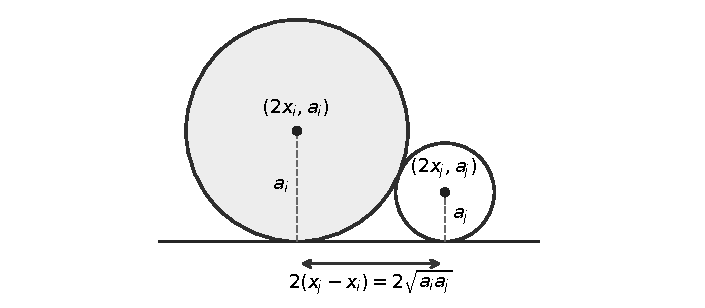
\includegraphics[width=.65\linewidth]{figures/line_geometry.pdf}
\caption{Two disks resting on a line, with horizontal center coordinates
$2x_i$ and $2x_j$. At contact their squared center separation is
$4(x_j-x_i)^2+(a_j-a_i)^2=(a_i+a_j)^2$, giving equality in~\eqref{eq:line}.}
\label{fig:line}
\end{figure}

For a fixed left-to-right word $w=(w_1,\ldots,w_N)$ its least span
$\ell(w)$ is given by
\begin{equation}\label{eq:recurrence}
 x_1=0,\qquad x_i=\max_{j<i}\{x_j+\sqrt{w_iw_j}\},\qquad \ell(w)=x_N.
\end{equation}
These coordinates are nondecreasing and satisfy every pair constraint.
Induction shows that any feasible ordered placement starting at zero
has its $i$th coordinate at least $x_i$. Thus $\ell(w)$ is the cost of
the longest increasing-index path from $1$ to $N$, and $b(a)$ is its
attained minimum over the orders. Deleting or decreasing marks cannot
increase $b$. Scaling every mark by $h\ge0$ scales $b$ by $h$.

\begin{lemma}[Bounded closing cost]\label{lem:closing}
Let $B(a)$ be the infimum circumference of a circle on which both arcs
between marks $i,j$ have length at least $\sqrt{a_i a_j}$. Then
$b(a)\le B(a)\le b(a)+M$. A gap of length $M$ also suffices to join
any two feasible line placements.
\end{lemma}
\begin{proof}
Cut a feasible circle to obtain a feasible line placement. Conversely,
join the two ends of an optimal line placement by a gap of length $M$.
For each pair, one arc is its line separation and the complementary
arc contains the gap. On joining two line placements the same gap
separates every cross pair, since $\sqrt{a_i a_j}\le M$.
\end{proof}

\begin{lemma}[Geometric comparison]\label{lem:profile-squeeze}
For $n\ge3$,
\begin{equation}\label{eq:profile-squeeze}
 \frac{b(a_n)}{\pi n}-\frac{M}{n}
 \ \le\ \frac{R_n}{N_n n}\ \le\ \frac{b(a_n)+M}{\pi n}.
\end{equation}
\end{lemma}
\begin{proof}
For $u,v\le N_n M$ and $R>0$, the two forms of~\eqref{eq:theta} give
\[
 \frac{2\sqrt{uv}}{R+N_nM}\le\theta_R(u,v)\le\frac{2\sqrt{uv}}{R}
\]
by $\asin z\ge z$ and $\atan z\le z$. Multiplying the angles of a
feasible ring by $(R+N_nM)/(2N_n)$ produces a circle feasible for
$B(a_n)$ with circumference $\pi(R/N_n+M)$. The lower comparison now
follows from Lemma~\ref{lem:closing}, taking the infimum over $R$.
For the upper comparison, rescale the circle of circumference $b(a_n)+M$
constructed in that lemma to angle $2\pi$. Each arc meets the upper
angular requirement at $R=N_n(b(a_n)+M)/\pi$. For $M=0$ both infima
are zero directly.
\end{proof}

\section{The limit law}\label{sec:profiles}

For a nondecreasing $Q:(0,1]\to[0,M]$, write
$b_n^Q=b(Q(1/n),\ldots,Q(1))$. Replicating a sampled list supplies every mark of a larger sampled
list after deletion and decrease.

\begin{lemma}[Replication of a quantile template]\label{lem:profile-copy}
If $m\ge n\ge2$ and $q=\lceil m/n\rceil$, then
\[
 b_m^Q\le q(b_n^Q+M)-M,\qquad
 \lim_{m\to\infty}\frac{b_m^Q}{m}=\inf_{n\ge2}\frac{b_n^Q+M}{n}.
\]
\end{lemma}
\begin{proof}
Join $q$ optimal copies by Lemma~\ref{lem:closing} and discard the
$d=nq-m$ smallest marks. The $i$th remaining mark in sorted order has
argument $\lceil(i+d)/q\rceil/n\ge i/m$, since
$m(i+d)-nqi=d(m-i)\ge0$. Decrease it to $Q(i/m)$. This assigns each
target once and preserves all separations, including ties. Dividing
the resulting span bound by $m$ and sending $m$ to infinity gives
$\limsup_m b_m^Q/m\le(b_n^Q+M)/n$ for every $n\ge2$. The infimum of
the right side is at most $\liminf_n b_n^Q/n$, since $M/n\to0$ and
$0\le b_n^Q\le(n-1)M$.
\end{proof}

For a probability law $\mu$ on $[0,M]$ let
$Q_\mu(t)=\inf\{x\in[0,M]:\mu([0,x])\ge t\}$, $0<t\le1$.
Define $E(\mu)$ by the limit in Lemma~\ref{lem:profile-copy} for
$Q=Q_\mu$.

\begin{theorem}[Radius-profile limit]\label{thm:profile-law}
Suppose $0\le a_{n,i}\le M<\infty$ for all $n,i$ and
$n^{-1}\sum_{i=1}^n\delta_{a_{n,i}}$ converges weakly to $\mu$.
For any sequence of scales $N_n>0$,
\[
 \frac{b(a_n)}{n}\longrightarrow E(\mu),\qquad
 \frac{R_n}{N_n n}\longrightarrow\frac{E(\mu)}{\pi}.
\]
In particular, a Riemann-integrable profile $f:[0,1]\to[0,M]$ sampled
at $i/n$ has limit law $\operatorname{law}(f(U))$ for $U$ uniform on $(0,1)$.
\end{theorem}
\begin{proof}
For two matched lists $a,c$ of $n$ marks in $[0,M]$,
\begin{equation}\label{eq:profile-change}
 |b(a)-b(c)|\le2\sqrt M\sum_i|\sqrt{a_i}-\sqrt{c_i}|.
\end{equation}
Each edge product changes by at most $\sqrt M$ times the sum of the
changes in its endpoint square roots. Each vertex occurs at most twice
as an endpoint on a path. Taking the longest path
in~\eqref{eq:recurrence} and then the minimum over orders preserves
this estimate.

Match the square roots of the sorted marks in $a_n$ to
$\sqrt{Q_\mu(i/n)}$. Their mean absolute distance equals the integral
over $[0,\sqrt M]$ of the absolute difference of the two empirical
distribution functions. At each threshold the sorted indicator lists
are nested, and integration counts the length of each matched interval.
At threshold $s$ the quantile sample counts $\lfloor n\mu([0,s^2])\rfloor$
entries. Its distribution function is thus within $1/n$ of
$\mu([0,s^2])$. The array distribution functions converge to this same
value at continuity points of the root-mark distribution. Bounded
convergence gives vanishing mean matched distance. The first limit now
follows from~\eqref{eq:profile-change} and Lemma~\ref{lem:profile-copy},
and the second follows from~\eqref{eq:profile-squeeze}. For the profile
statement, apply right-endpoint Riemann sums to each continuous test
function composed with $f$.
\end{proof}

For two laws $\mu,\nu$ on $[0,M]$, applying~\eqref{eq:profile-change}
to their quantile samples and taking Riemann sums gives
\[
 |E(\mu)-E(\nu)|\le2\sqrt M
 \int_0^1|\sqrt{Q_\mu(t)}-\sqrt{Q_\nu(t)}|\,dt.
\]
The integrand is Riemann integrable because both quantiles are bounded
and monotone. Monotonicity is needed only for the template. The given
marks may occur in any order.

\paragraph*{Two sampling examples}
Take $a_{n,i}=c$ for odd $i$ and $0$ for even $i$, where $c>0$.
The empirical law tends to $\mu=(\delta_0+\delta_c)/2$. The $h=\lceil n/2\rceil$
positive marks require span at least $c(h-1)$, attained by spacing them
$c$ apart and placing the zeros at the first point. Thus $E(\mu)=c/2$ and
the normalized ring radius tends to $c/(2\pi)$. For a different
example, take $f=\mathbf1_{\mathbb Q}$ on $[0,1]$. The random
variable $f(U)$ vanishes almost surely, but every grid mark $f(i/n)$
is one. Their line span is $n-1$, so the ring coefficient is $1/\pi$.
For a measurable $f$ the sampled law agrees with the proposed law of
$f(U)$ precisely when $n^{-1}\sum_{i=1}^n g(f(i/n))\to\int_0^1g(f(t))\,dt$
for every continuous $g$ on $[0,M]$.

\begin{corollary}[Uniform marks and consecutive integer radii]\label{thm:existence}
For the uniform law on $[0,1]$, put $b_n=b(1/n,\ldots,1)$ and
$E=E(\operatorname{law}(U))$. For outer radii $1,\ldots,n$,
\begin{equation}\label{eq:limit}
 \Rstar(n)=\CC n^2+o(n^2),\qquad
 \pi\CC=E=\lim_{n\to\infty}\frac{b_n}{n}=\inf_{n\ge2}\frac{b_n+1}{n}.
\end{equation}
For $n\ge3$ the finite comparison is
\begin{equation}\label{eq:squeeze}
 \frac{b_n}{\pi n}-\frac1n\le\frac{\Rstar(n)}{n^2}\le\frac{b_n+1}{\pi n}.
\end{equation}
\end{corollary}
\begin{proof}
Use $Q(t)=t$, $M=1$ and $N_n=n$ in Lemma~\ref{lem:profile-copy},
Theorem~\ref{thm:profile-law} and~\eqref{eq:profile-squeeze}.
At least $n/2$ marks are at least $1/2$, with successive separations
at least $1/2$ in their induced order. Thus $E\ge1/4$ and $\CC>0$.
\end{proof}
